\documentclass[11pt]{article}

% Packages
\usepackage{graphicx}   % for pictures
\usepackage{amsthm}     % for math
\usepackage{amsmath, mathtools}    %   more math
\usepackage{amsfonts}   %   more math
\usepackage{physics}    % more symbols
\usepackage{circuitikz} % for circuit diagrams
\usepackage{amssymb}    % math symbols
\usepackage{siunitx}    % units
\usepackage{mathrsfs}   % fancy text
\usepackage{color}      % colored letters for notes and reminders
\usepackage{float}      % for image location

%The amsthm package lets you format different types of mathematical ideas nicely. You use it by defining "\newtheorem"s as below:
\newtheorem{problem}{Problem}
\newtheorem{theorem}{Theorem}
\newtheorem*{proposition}{Proposition}
\newtheorem{lemma}[theorem]{Lemma}
\newtheorem{corollary}[theorem]{Corollary}
\theoremstyle{definition}
\newtheorem{defn}[theorem]{Definition}

% Magins

\setlength{\voffset}{0.1in}
\setlength{\paperwidth}{8.5in}
\setlength{\paperheight}{11in}
\setlength{\headheight}{14pt}
\setlength{\headsep}{0.5in}
\setlength{\textheight}{11in}
\setlength{\textheight}{8in}
\setlength{\topmargin}{-0.25in}
\setlength{\textwidth}{7in}
\setlength{\topskip}{0in}
\setlength{\oddsidemargin}{-0.25in}
\setlength{\evensidemargin}{-0.25in}

% For images in this document:
\graphicspath{ {images/} }

% User Defined Commands
\newcommand{\nder}[2]{\frac{d^{#1} #2}{d t^{#1}}}   % The nth derivative wrt t: {n}{x(t)}
\newcommand{\der}[1]{\frac{d #1}{d t}}              % Derivative wrt t: {x(t)}
\newcommand{\infint}{\int_{-\infty}^{\infty}}       % Integral from - infinity to + infinity
\newcommand{\infsum}[1]{\sum_{#1 = -\infty}^{\infty}}% Sum of a variable from - to + infinity
\newcommand{\para}[1]{\left( #1 \right)}            % Instead of writing parenthesis all the time

% User Command for Wider Matrices
\makeatletter
\renewcommand*\env@matrix[1][\arraystretch]{%
  \edef\arraystretch{#1}%
  \hskip -\arraycolsep
  \let\@ifnextchar\new@ifnextchar
  \array{*\c@MaxMatrixCols c}}
\makeatother


% Heading:
\usepackage{fancyhdr}
\pagestyle{fancy}
\lhead{Nicholas Pham}
\chead{ES 155}          %   Change the Class!!
\rhead{Homework 2}   %   Change the Problem Set Number!!


% ----- BEGIN DOCUMENT-----
\begin{document}

\textbf{\huge{ES 155 Homework 2}}    %   Change the Class and Problem Set Number!!
\normalsize

\begin{enumerate}
    \item % Problem 1
    In this system model where $H(t)$ represents the population of hares and $G(t)$ represents the population of tigers at time $t$, the population dynamics of the system are given by

    \begin{align}
        \frac{d}{dt} H(t) &= r H(t) - a G(t) \\
        \frac{d}{dt} G(t) &= \frac{b H(t) G(t)}{c + H(t)} - e G(t)
    \end{align}

    where $H(t) \leq 0$ and $G(t) \leq 0$ (a population can't be negative).  In this model, $r$ is the growth coefficient of the hares, $a$ is the diminishing coefficient on the hares by the tigers, $b$ is the growth coefficient of the tigers, $c$ is a constant controlling prey consumption when there is low hare population, and $e$ represents the mortality rate of the tigers.

    \begin{enumerate}
        \item % Part a
        The equilibrium points of this system satisfy the condition $\begin{bmatrix} \frac{d}{dt} H(t) \\ \frac{d}{dt} G(t) \end{bmatrix} = 0$:

        \begin{align}
            \frac{d}{dt} H(t) &= r H(t) - a G(t) = 0 \quad \text{solving for $G$} \\
            G(t) &= \frac{r}{a} H(t) \quad \quad \text{plug into $\frac{d}{dt}G(t)$}\\
            \frac{d}{dt} G(t) &= \frac{b H(t) G(t)}{c + H(t)} - e G(t) = 0 = \frac{b H(t) \frac{r}{a} H(t) }{c + H(t)} - e \frac{r}{a} H(t) \\
            \frac{br}{a} H^2(t) &= \frac{er}{a} H(t) \left( c + H(t) \right) \\
            0 &= (b - e) \frac{r}{a} H^2(t) - \frac{erc}{a}H(t) \\
            H^* &= \frac{ec}{b - e}, 0 \quad \quad \text{plug back in} \\
            G^* &= \frac{r}{a} \left( \frac{ec}{b-e} \right), 0
        \end{align}

        There are two equilibirium points: $\begin{bmatrix} H^* \\ G^* \end{bmatrix} = \begin{bmatrix} \frac{ec}{b - e} \\ \frac{r}{a} \left( \frac{ec}{b-e} \right) \end{bmatrix}, \begin{bmatrix} 0 \\ 0 \end{bmatrix}$.


        \item % Part b
        Let $r = 0.1, e = 0.1, c = 100, b = 0.2, a = 0.5$.  To linearize the system, first find numeric values for the equilibirum points.  Pluging these constants into the answer for part (a) gives 

        \begin{align}
            \begin{bmatrix} H^* \\ G^* \end{bmatrix} &= \begin{bmatrix} \frac{ec}{b - e} \\ \frac{r}{a} \left( \frac{ec}{b-e} \right) \end{bmatrix}, \begin{bmatrix} 0 \\ 0 \end{bmatrix} = \begin{bmatrix} 100 \\ 20  \end{bmatrix}, \begin{bmatrix} 0 \\ 0 \end{bmatrix}
        \end{align}

        Next, write down the $A, B, C, D$ matrices.  In this case, there is no control input yet, so $B$ and $D$ are 0.  We also don't care about the output $y$ now, which is not defined, so only A needs to be considered.

        \begin{align}
            \frac{d}{dt} x(t) = \begin{bmatrix}[1.5] \frac{\partial f_H}{\partial H} &  \frac{\partial f_H}{\partial G} \\ \frac{\partial f_G}{\partial H} &  \frac{\partial f_G}{\partial G}  \end{bmatrix} \begin{bmatrix} H(t) - H^* \\ G(t) - G^* \end{bmatrix}\\
            A &= \begin{bmatrix} r & -a \\ \frac{bc G^*}{\left( c + H^* \right)^2} & \frac{b H^*}{c + H^*} - e \end{bmatrix}
        \end{align}

        Plugging in the constants and the two equilibrium points $(100, 20)$ and $(0, 0)$, repectively, we get

        \begin{align}
            A &= \begin{bmatrix} 0.1 & -0.5 \\ 0.01 & 0 \end{bmatrix}, \begin{bmatrix} 0.1 & -0.5 \\ 0.002 & -0.1 \end{bmatrix}
        \end{align}

        Now define $\tilde{x} = \begin{bmatrix} \tilde{H}(t) \\ \tilde{G}(t) \end{bmatrix} = \begin{bmatrix} H(t) - H^* \\ G(t) - G^* \end{bmatrix}$.  For the two equilibrium points, we have

        \begin{align}
            \begin{bmatrix} \tilde{H}(t) \\ \tilde{G}(t) \end{bmatrix} &= \begin{bmatrix} H(t) - H^* \\ G(t) - G^* \end{bmatrix} = \begin{bmatrix} H(t) - 100 \\ G(t) - 20 \end{bmatrix}, \begin{bmatrix} H(t) \\ G(t) \end{bmatrix}
        \end{align}

        Therefore, the linearized model for the system is:

        \begin{align}
            \begin{bmatrix} \dot{\tilde{H}}(t) \\ \dot{\tilde{G}}(t) \end{bmatrix} &= \begin{bmatrix} 0.1 & -0.5 \\ 0.01 & 0 \end{bmatrix} \begin{bmatrix} \tilde{H}(t) \\ \tilde{G}(t) \end{bmatrix} , \begin{bmatrix} 0.1 & -0.5 \\ 0.002 & -0.1 \end{bmatrix} \begin{bmatrix} \tilde{H}(t) \\ \tilde{G}(t) \end{bmatrix} 
        \end{align}

        for equilibirum points $(100, 20)$ and $(0, 0)$ respectively.
        \item % Part c
        The eigenvalues of the Jacobian matrix $A$ indicate the stability of the system.  For the nonzero equilibrium point $(100, 20)$, the eigenvalues of the $A = \begin{bmatrix} 0.1 & -0.5 \\ 0.01 & 0 \end{bmatrix}$ are $0.05 \pm 0.05 i$.  Because the real part of both eigenvalues is positive, this equilibrium is unstable.

        The eigenvalues of the Jacaboian matrix $A = \begin{bmatrix} 0.1 & -0.5 \\ 0.002 & -0.1 \end{bmatrix}$ corresponding to the equilibrium point $(0, 0)$ are $\pm 0.949$.  Again, because one of these eigenvalues is positive, the equilibrium point is unstable.

        Note: See attached MATALB code for eigenvalue calcualtion.

        \item % Part d
        By adding a control input $u(t)$ to the system, we have

        \begin{align}
            \dot(x) &= Ax + u(t) \quad \text{with} \quad u(t) = \begin{bmatrix} \omega \cdot \big( H(t) - H^* \big) \\ 0 \end{bmatrix}
        \end{align}

        Using only the nonzero equilibrium point $(100, 20)$, we can write the system in the form $\dot{x} = Ax + u(t)$:

        \begin{align}
            \dot{x}(t) &= \begin{bmatrix} 0.1 & -0.5 \\ 0.01 & 0 \end{bmatrix} \begin{bmatrix} H(t) - 100 \\ G(t) - 20 \end{bmatrix} + \begin{bmatrix} \omega \cdot \big( H(t) - H^* \big) \\ 0 \end{bmatrix}
        \end{align}

        This can also be rewritten in an autonomous form $\dot{x} = \bar{A}x$, which just involves adding $\omega$ to the first entry in $A$:

        \begin{align}
            \dot{x}(t) &= \begin{bmatrix} 0.1 + \omega & -0.5 \\ 0.01 & 0 \end{bmatrix} \begin{bmatrix} H(t) - 100 \\ G(t) - 20 \end{bmatrix}
        \end{align}

        For $\omega = -0.61$, the stability of the system can be determined by looking at the eigenvalues of $\bar{A}$:

        \begin{align}
            \bar{A} &= \begin{bmatrix} -0.51 & -0.5 \\ 0.01 & 0 \end{bmatrix} \\
            \texttt{eig} \big( \bar{A} \big) &= -0.5, -0.01
        \end{align}

        Because the real parts of both eigenvalues are negative, the system is stable.  Adding this control input stabalized the system.

    \end{enumerate}

    \item % Problem 2
    The given dynamical equations for the cart inverted pendulum system are

    \begin{align}
        (M + m)\ddot{p} - ml \cos (\theta) \ddot{\theta} + c \dot{p} + ml \sin (\theta) \dot{\theta}^2 &= F \label{eqn:3a}\\
        -ml \cos (\theta) \ddot{p} + \left( I + ml^2 \right) \ddot{\theta} + \gamma \dot{\theta} - mgl \sin (\theta) &= 0 \label{eqn:3b}
    \end{align}

    \begin{enumerate}
        \item % Part a

        To derive the state space model in terms of $\dot{x} = f(x,u), y = h(x, u)$ with control input $u = F$, output $y = \begin{bmatrix} p \\ \theta \end{bmatrix}$ and $x = \begin{bmatrix} p \\ \theta \\ \dot{p} \\ \dot{\theta} \end{bmatrix}$ and parameters $L, M, m, I, g, c$, first find $\dot{x}$:

        \begin{align}
            \dot{x} &= \frac{d}{dt}\begin{bmatrix} p \\ \theta \\ \dot{p} \\ \dot{\theta} \end{bmatrix} = \begin{bmatrix} \dot{p} \\ \dot{\theta} \\ \ddot{p} \\ \ddot{\theta} \end{bmatrix}
        \end{align}

        The first two rows are easy.  To find $\ddot{p}$, solve for $\ddot{\theta}$ in equation \ref{eqn:3b} then plug into equation \ref{eqn:3a}.

        \begin{align}
            \ddot{\theta} &= \frac{1}{I + ml^2} \big( ml \cos (\theta) \ddot{p} - \gamma \dot{\theta} + mgl \sin (\theta) \big) \\
            u &= (M + m)\ddot{p} - ml \cos (\theta) \frac{ml \cos (\theta) \ddot{p} - \gamma \dot{\theta} + mgl \sin (\theta)}{I + ml^2}  + c \dot{p} + ml \sin (\theta) \dot{\theta}^2 \\
            \ddot{p} &= \frac{u - ml \sin(\theta) \dot{\theta}^2 - c \dot{p} - ml \cos(\theta) \frac{\gamma}{I + ml^2} \dot{\theta} + \frac{ m^2 g l^2}{I + ml^2} \cos (\theta) \sin (\theta)}{M + m - \frac{m^2 l^2 \cos^2 (\theta)}{I + ml^2}}
        \end{align}

        Similarly, solve for $\ddot{p}$ in equation \ref{eqn:3a} then plug into equation \ref{eqn:3b}.

        \begin{align}
            \ddot{p} &= \frac{1}{M + m} \left( u + ml \cos (\theta) \ddot{\theta} - c \dot{p} - ml \sin (\theta) \dot{\theta}^2 \right) \\
            0 &= -ml \cos (\theta) \frac{u + ml \cos (\theta) \ddot{\theta} - c \dot{p} - ml \sin (\theta) \dot{\theta}^2}{M + m}  + \left( I + ml^2 \right) \ddot{\theta} + \gamma \dot{\theta} - mgl \sin (\theta) \\
            \ddot{\theta} &= \frac{ml \cos (\theta)u - ml \cos (\theta) c \dot{p} - m^2 l^2 \cos (\theta) \sin (\theta) \dot{\theta}^2 - (M + m)(\gamma \dot{\theta} - mgl \sin (\theta))}{(M + m)(I + ml^2) - l^2 \cos^2(\theta)}
        \end{align}

        Therefore, the state space model for this system can be written

        \begin{align}
            \dot{x} &= \begin{bmatrix} \dot{p} \\ \dot{\theta} \\ \ddot{p} \\ \ddot{\theta} \end{bmatrix} = \begin{bmatrix}[1.5] \dot{p} \\ \dot{\theta} \\ \frac{u - ml \sin(\theta) \dot{\theta}^2 - c \dot{p} - ml \cos(\theta) \frac{\gamma}{I + ml^2} \dot{\theta} + \frac{ m^2 g l^2}{I + ml^2} \cos (\theta) \sin (\theta)}{M + m - \frac{m^2 l^2 \cos^2 (\theta)}{I + ml^2}} \\  \frac{ml \cos (\theta)u - ml \cos (\theta) c \dot{p} - m^2 l^2 \cos (\theta) \sin (\theta) \dot{\theta}^2 - (M + m)(\gamma \dot{\theta} - mgl \sin (\theta))}{(M + m)(I + ml^2) - l^2 \cos^2(\theta)} \end{bmatrix} \label{eqn:xdot}\\
            y &= \begin{bmatrix} p \\ \theta \end{bmatrix}
        \end{align}

        \item % Part b
        To find the equilibrium points for $F = 0$, set $\dot{x} = 0$.  By equation \ref{eqn:xdot}, we can immediately see that $\dot{p} = 0$ and $\dot{\theta} = 0$.  Plugging this into the last two entries of $\dot{x}$ gives

        \begin{align}
            \ddot{p} &= \frac{\frac{ m^2 g l^2}{I + ml^2} \cos (\theta) \sin (\theta)}{M + m - \frac{m^2 l^2 \cos^2 (\theta)}{I + ml^2}} = 0 \\
            \ddot{\theta} &= \frac{(M + m) mgl \sin (\theta)}{(M + m)(I + ml^2) - l^2 \cos^2(\theta)} = 0
        \end{align}

        The latter equation implies that $\sin (\theta) = 0$ so $\theta  = n \pi \forall n \in \mathbb{Z}$, which means that the cart-inverted pedulum has an equilibrium point at both the vertical top and bottom of the pendulum's swing.  The prior equation agrees with this, as there is also a $\sin (\theta)$ multiplier.  Note that the $p$ position does not matter for either the dynamic equations or the equilibirium points, which makes sense: the system is "position invariant" in that offsets in position will not affect the dynamics.  Thus, the system dynamics can be calculated for two equilibrium points:

        \begin{align}
            x &= \begin{bmatrix} p \\ \theta \\ \dot{p} \\ \dot{\theta} \end{bmatrix} = \begin{bmatrix} p^* \\ 0 \\ 0 \\ 0 \end{bmatrix}, \begin{bmatrix} p^* \\ \pi \\ 0 \\ 0 \end{bmatrix}
        \end{align}

        where $ \forall \quad p^* \in \mathbb{R}$.

        Now to linearize the system near these two points, we must write the Jacobian matrix $A$ for the system.

        \begin{align}
            \dot{x} &= Ax = \begin{bmatrix}[1.5]
                \frac{\partial f_p}{\partial p} & \frac{\partial f_p}{\partial \theta} & \frac{\partial f_p}{\partial \dot{p}} & \frac{\partial f_p}{\partial \dot{\theta}} \\
                 \frac{\partial f_{\theta}}{\partial p} & \frac{\partial f_{\theta}}{\partial \theta} & \frac{\partial f_{\theta}}{\partial \dot{p}} & \frac{\partial f_{\theta}}{\partial \dot{\theta}} \\ 
                 \frac{\partial f_{\dot{p}}}{\partial p} & \frac{\partial f_{\dot{p}}}{\partial \theta} & \frac{\partial f_{\dot{p}}}{\partial \dot{p}} & \frac{\partial f_{\dot{p}}}{\partial \dot{\theta}} \\ 
                 \frac{\partial f_{\dot{\theta}}}{\partial p} & \frac{\partial f_{\dot{\theta}}}{\partial \theta} & \frac{\partial f_{\dot{\theta}}}{\partial \dot{p}} & \frac{\partial f_{\dot{\theta}}}{\partial \dot{\theta}}
             \end{bmatrix}
             \begin{bmatrix}
                p \\ \theta \\ \dot{p} \\ \dot{\theta}
             \end{bmatrix}\\
        \end{align}

        At these two equilibrium points, where $\theta = 0, \pi$, we can make some similifying assumptions.  For $\theta = 0$, we can approximate $\sin\theta \approx \theta = 0$ and $\cos\theta \approx = 1$.  For $\theta = \pi$, we can approximate $\sin\theta \approx \pi - \theta$ and $\cos\theta \approx -1$.  With these approximations, we can write 

        \begin{align}
             A_{\theta^* = 0} &= \begin{bmatrix}[1.5]
                0 & 0 & 1 & 0 \\
                0 & 0 & 0 & 1 \\
                0 & \frac{m^2 l^2 g}{(M - m)(I + ml^2) - m^2 l^2} & -\frac{c (I + ml^2)}{(M - m)(I + ml^2) - m^2 l^2} & -\frac{\gamma lm}{(M - m)(I + ml^2) - m^2 l^2} \\
                0 & \frac{(M + m)mgl}{(M - m)(I + ml^2) - m^2 l^2} & -\frac{clm}{(M - m)(I + ml^2) - m^2 l^2} & -\frac{\gamma (M + m)}{(M - m)(I + ml^2) - m^2 l^2}
             \end{bmatrix} \\
            A_{\theta^* = \pi} &= \begin{bmatrix}[1.5]
                0 & 0 & 1 & 0 \\
                0 & 0 & 0 & 1 \\
                0 & \frac{m^2 l^2 g}{(M - m)(I + ml^2) - m^2 l^2} & -\frac{c (I + ml^2)}{(M - m)(I + ml^2) - m^2 l^2} & \frac{\gamma lm}{(M - m)(I + ml^2) - m^2 l^2} \\
                0 & -\frac{(M + m)mgl}{(M - m)(I + ml^2) - m^2 l^2} & \frac{clm}{(M - m)(I + ml^2) - m^2 l^2} & -\frac{\gamma (M + m)}{(M - m)(I + ml^2) - m^2 l^2}
             \end{bmatrix}
        \end{align}

        The difference between these two Jacobians is only the sign of some of the entries.

        To complete the system model, we need to write $B, C, D$.  Because the control input $F = u = 0$, $B = 0$ as well.  The $C$ matrix to get $y$ is simple because $y$ is just the first two entries of $x$, so 

        \begin{align}
            C &= \begin{bmatrix} 1 & 0 & 0 & 0 \\ 0 & 1 & 0 & 0 \end{bmatrix}
        \end{align}

        and $D$ is also 0.  With these matricies the system model can be written in the form

        \begin{align}
            \dot{x} &= Ax + Bu\\
            y &= Cx + Du
        \end{align}


        \item % Part c
        We can plug in the parameters to determine the stability of the system at the two equilibrium points.  One quantity that showed up often is $(M - m)(I + ml^2) - m^2 l^2$, which for the given parameters $M = 10 \text{ kg}, m = 80 \text{ kg}, I = 100 \text{ kg}\text{ m}^2$, and $L = 1 \text{ m}$ is $-19000 \text{ kg}^2 \text{ m}^2$.

        \begin{align}
             A_{\theta^* = 0} &= \begin{bmatrix}
             0 & 0 & 1.0 & 0\\
             0 & 0 & 0 & 1.0\\
             0 & 6.4 & -0.00184 & -8.16 \times {10}^{-5}\\
             0 & 7.2 & -8.16\ \times {10}^{-4} & -9.18 \times {10}^{-5} 
             \end{bmatrix} \\
        \end{align}

        \begin{align}
             A_{\theta^* = \pi} &= \begin{bmatrix}
             0 & 0 & 1.0 & 0\
             0 & 0 & 0 & 1.0\\
             0 & 6.4 & -0.00184 & 8.16 \times {10}^{-5}\\
             0 & -7.2 & 8.16 \times {10}^{-4} & -9.18 \times {10}^{-5} 
             \end{bmatrix} \\
        \end{align}

        Taking the eigenvalues of these matrices, we can determine the stability of each of these equilibirium points.  Plugging into MATLAB gives the eigenvalues of $A_{\theta = 0}$ as    

        \begin{align*}
            \begin{matrix}
                 0 \\
            2.6829 \\
           -2.6837 \\
           -0.0011
            \end{matrix}
        \end{align*}

        This shows that the upright pendulum is unstable, as we would expect.  When plugging in the eigenvalues of $A_{\theta = \pi}$ I got

        \begin{align*}
            \begin{matrix}
               0.0000 + 0.0000i \\
              -0.0004 + 2.6833i \\
              -0.0004 - 2.6833i \\
              -0.0011 + 0.0000i
            \end{matrix}
        \end{align*}

        This implies that this equilibrium point likely stable, though there is an eigenvalue with real part equal to zero which may complicate things.

        \item % Part d
        Examining the equilibrium point with $\theta = 0$ and defining state feedback $F = -Kx$ for $K = [ -15.3, 1730, -50, 443]$.  We can examine the stability of the system with the addition of the feedback by examining the eigenvalues of $\bar{A}$:

        \begin{align}
            \dot{x} &= Ax + Bu = Ax + B(-Kx) = (A - BK)x = \bar{A}x\\
            \bar{A} &= (A - BK)
        \end{align}

        Previously we had $B = \begin{bmatrix} 0 \\ 0 \\ \frac{I + ml^2}{(M - m)(I + ml^2) - m^2 l^2} \\ \frac{lm}{(M - m)(I + ml^2) - m^2 l^2} \end{bmatrix}$.  With the given parameters, $B = \begin{bmatrix} 0 \\ 0 \\ 0.0184 \\ 0.0082 \end{bmatrix}$.  Now we can compute $\bar{A}$.

        \begin{align}
            \bar{A} &= A - BK = \begin{bmatrix} 0 & 0 & 1.0 & 0\\
                                                0 & 0 & 0 & 1.0\\ 
                                                0.281 & -25.4 & 0.917 & -8.14\\ 
                                                0.125 & -6.92 & 0.407 & -3.62  \end{bmatrix}
        \end{align}

        This matrix now describes the system with the feedback control: $\dot{x} = \bar{A}x$.  Its eigenvalues are

        \begin{align*}
            \begin{matrix}
              -0.9994 + 1.9990i \\
              -0.9994 - 1.9990i \\
              -0.3506 + 0.3495i \\
              -0.3506 - 0.3495i
            \end{matrix}
        \end{align*}

        Because the real part of all the eigenvalues are negative, the system is now stable.  Adding the feedback controller stabalized the system.

        \item % Part e
        Simulating the nonlinear system in MATLAB can show the local effectiveness of the stabilization feedback control.  Using Equation \ref{eqn:xdot} and calculating $F = u = -Kx$ as in part (d), I simulated the system using \texttt{ode45}.

        However, unlike the linearization of the system $\dot{x} = A_bar x$ which always remains stable despite the initial condition, the nonlinear model only stabalizes for certain initial conditions.  For example, Figure \ref{fig:cart_stable} shows the system with initial condition $x_0 = \begin{bmatrix} 0 \\ 0.5 \\ 0 \\ 0 \end{bmatrix}$.  In this case, the system stabilizes.  However, Figure \ref{fig:cart_unstable} shows the system with initial condition $x_0 = \begin{bmatrix} 0 \\ 1 \\ 0 \\ 0 \end{bmatrix}$.  In this case, the system is unstable, as the feedback control cannot keep up.

        \begin{figure}
            \centering
            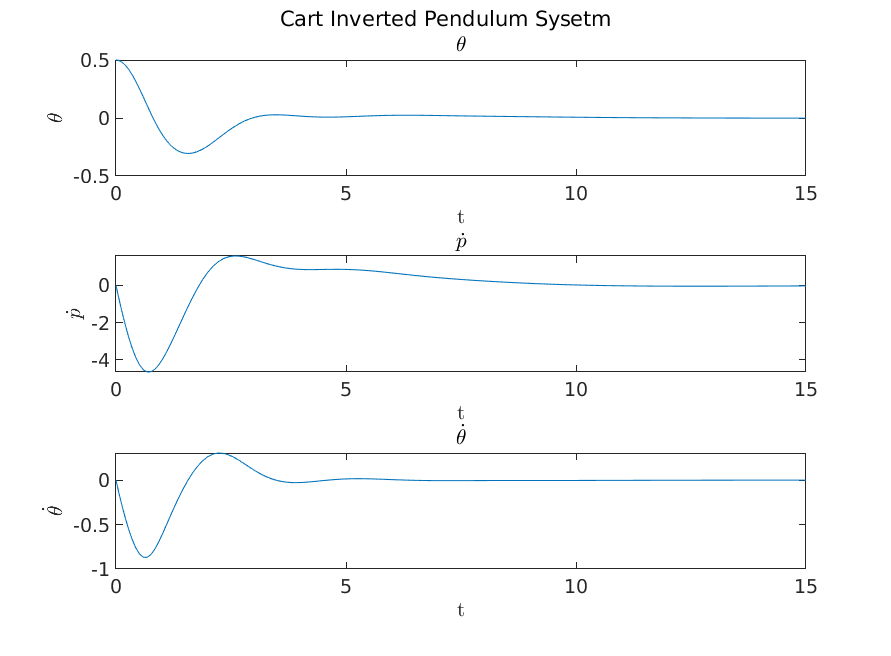
\includegraphics[width = \textwidth]{StableIC_0_05_0_0.png}
            \caption{Stable Cart Inverted Pendulum with initial condition $x_0 = \begin{bmatrix} 0 \\ 0.5 \\ 0 \\ 0 \end{bmatrix}$ }
            \label{fig:cart_stable}
        \end{figure}

        \begin{figure}
            \centering
            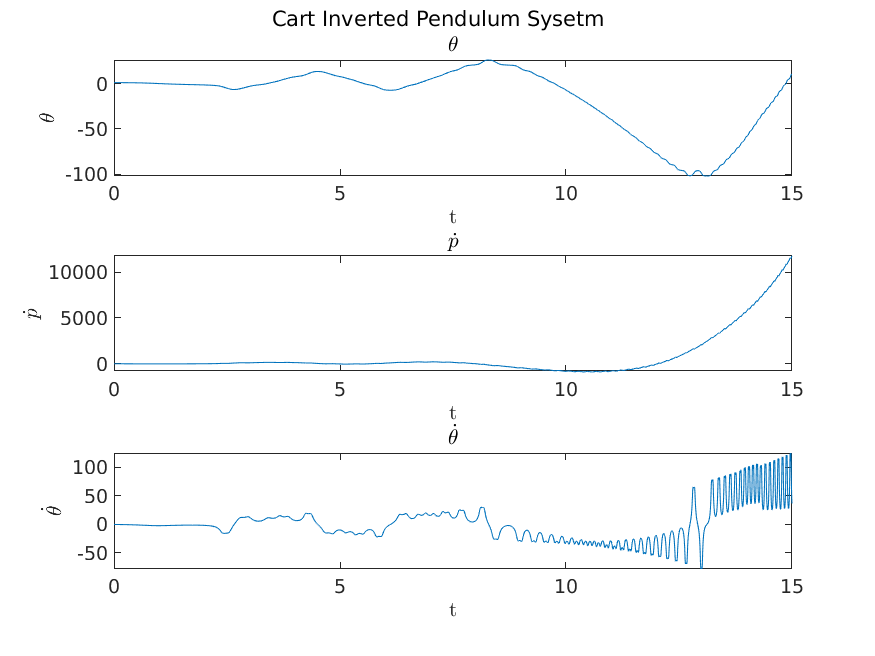
\includegraphics[width = \textwidth]{UnstableIC_0_1_0_0.png}
            \caption{Unstable Cart Inverted Pendulum with initial condition $x_0 = \begin{bmatrix} 0 \\ 1 \\ 0 \\ 0 \end{bmatrix}$}
            \label{fig:cart_unstable}
        \end{figure}

    \end{enumerate}

\end{enumerate}
\end{document}


